\documentclass[letterpaper]{article}
\usepackage[margin=1in]{geometry}
\usepackage[utf8]{inputenc}
\usepackage{textcomp}
\usepackage{amssymb}
\usepackage{natbib}
\usepackage{graphicx}
\usepackage{gensymb}
\usepackage{amsthm, amsmath, mathtools}
\usepackage[dvipsnames]{xcolor}
\usepackage{enumerate}
\usepackage{mdframed}
\usepackage[most]{tcolorbox}
\usepackage{csquotes}
% https://tex.stackexchange.com/questions/13506/how-to-continue-the-framed-text-box-on-multiple-pages

\tcbuselibrary{theorems}

\newcommand{\R}{\mathbb{R}}
\newcommand{\Z}{\mathbb{Z}}
\newcommand{\N}{\mathbb{N}}
\newcommand{\Q}{\mathbb{Q}}
\newcommand{\C}{\mathbb{C}}
\newcommand{\code}[1]{\texttt{#1}}
\newcommand{\mdiamond}{$\diamondsuit$}
\newcommand{\PowerSet}{\mathcal{P}}
\newcommand{\Mod}[1]{\ (\mathrm{mod}\ #1)}
\DeclareMathOperator{\lcm}{lcm}

%\newtheorem*{theorem}{Theorem}
%\newtheorem*{definition}{Definition}
%\newtheorem*{corollary}{Corollary}
%\newtheorem*{lemma}{Lemma}
\newtheorem*{proposition}{Proposition}


\newtcbtheorem[number within=section]{theorem}{Theorem}
{colback=green!5,colframe=green!35!black,fonttitle=\bfseries}{th}

\newtcbtheorem[number within=section]{definition}{Definition}
{colback=blue!5,colframe=blue!35!black,fonttitle=\bfseries}{def}

\newtcbtheorem[number within=section]{corollary}{Corollary}
{colback=yellow!5,colframe=yellow!35!black,fonttitle=\bfseries}{cor}

\newtcbtheorem[number within=section]{lemma}{Lemma}
{colback=red!5,colframe=red!35!black,fonttitle=\bfseries}{lem}

\newtcbtheorem[number within=section]{example}{Example}
{colback=white!5,colframe=white!35!black,fonttitle=\bfseries}{def}

\newtcbtheorem[number within=section]{note}{Important Note}{
        enhanced,
        sharp corners,
        attach boxed title to top left={
            xshift=-1mm,
            yshift=-5mm,
            yshifttext=-1mm
        },
        top=1.5em,
        colback=white,
        colframe=black,
        fonttitle=\bfseries,
        boxed title style={
            sharp corners,
            size=small,
            colback=red!75!black,
            colframe=red!75!black,
        } 
    }{impnote}
\usepackage[utf8]{inputenc}
\usepackage[english]{babel}
\usepackage{fancyhdr}
\usepackage[hidelinks]{hyperref}

\pagestyle{fancy}
\fancyhf{}
\rhead{CSE 105}
\chead{Monday, February 14, 2022}
\lhead{Lecture 11}
\rfoot{\thepage}

\setlength{\parindent}{0pt}

\begin{document}

\section{Turing Machines (3.1)}
First proposed by Alan Turing in 1936, the \textbf{Turing machine} is a much more accurate model of a general purpose computer. It can do everything that a real computer can do, but even it cannot solve certain problems\footnote{In a very real sense, these problems are beyond the theoretical limits of computation.}.

\subsection{The Idea}
\begin{itemize}
    \item The input string is \emph{written} on the leftost squares of the tape. The rest of the tape is empty. 
    \item We can read \emph{and} write on the tape. The read/write head starts at the leftmost position on the tape. 
    \item Computation proceeds according to the transition function. In other words, given the current state of machine, and the current symbol being read, the machine will 
    \begin{itemize}
        \item Transition to a new state.
        \item Write a symbol to its current position, overwriting the existing symbol.
        \item Moves the tape head $L$ or $R$. 
    \end{itemize}
    \item Computation ends if and when it enters either the \textbf{accept} or the \textbf{reject} state. This means that we can have programs that can run forever. 
\end{itemize}

\subsection{Language of a Turing Machine}
Given a Turing machine $M$, the language $L(M)$ is the set of all strings $w$ such that the computation of $M$ on $w$ \emph{halts} after entering the accept state. That is, $L(M) = \{w \mid w \text{ is accepted by } M\}$.

\subsection{Formal Definition}
As usual, the most important thing about the Turing machine is the transition function 
\[\delta: Q \times \Gamma \mapsto Q \times \Gamma \times \{L, R\}\]
That is, when the machine is in a certain state $q$ and the head is over a tape square containing the symbol $a$, and if $\delta(q, a) = (r, b, L)$, then the machine writes the symbol $b$ replacing the $a$, and goes to state $r$. The third component is either $L$ or $R$, and indicates whether the head moves to the left or right after writing. In this case, the $L$ indicates that we move the tape to the left. 

\begin{definition}{Turing Machine}{}
    A \textbf{Turing machine} is a 7-tuple $(Q, \Sigma, \Gamma, \delta, q_0, q_{\text{accept}}, q_{\text{reject}})$ where $Q, \Sigma, \Gamma$ are all finite sets and 
    \begin{enumerate}
        \item $Q$ is the set of states.
        \item $\Sigma$ is the input alphabet not containing the \emph{blank symbol} $\sqcup$.
        \item $\Gamma$ is the tape alphabet, where $\sqcup \in \Gamma$ and $\Sigma \subseteq \Gamma$. 
        \item $\delta: Q \times \Gamma \mapsto Q \times \Gamma \times \{L, R\}$ is the transition function. 
        \item $q_0 \in Q$ is the start state. 
        \item $q_{\text{accept}} \in Q$ is the accept state.
        \item $q_{\text{reject}} \in Q$ is the reject state, where $q_{\text{reject}} \neq q_{\text{accept}}$.   
    \end{enumerate} 
\end{definition}

\subsection{Configuration of a Turing Machine}
As a Turing machine computes, changes occur in the current state, the current tape contents, and the current head location. A setting of these three items is called a \textbf{configuration} of the Turing machine. They are often represented in a special way. For a state $q$ and two strings $u$ and $v$ over the tape alphabet $\Gamma$, we write $uqv$ for the configuration where the current state is $q$, the current tape contents is $uv$, and the current head location is the first symbol of $v$. 

\bigskip 

For example, $\code{1011}q_7\code{01111}$ represents the configuration when the tape is \code{101101111}, the current state is $q_7$, and the head is currently on the second \code{0}.
\begin{center}
    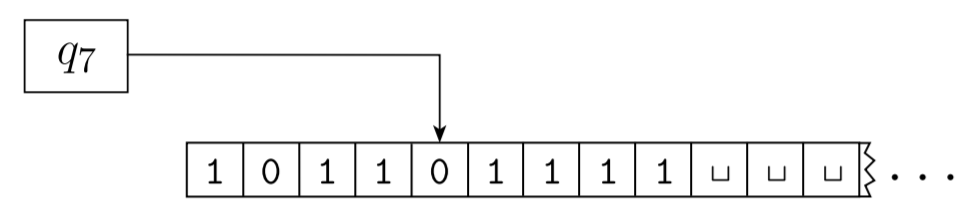
\includegraphics[scale=0.5]{../assets/turing_config_1.png}

    \textbf{Figure:} The configuration $\code{1011}q_7\code{01111}$. 
\end{center}

\subsubsection{Transitioning Between Configurations}
Suppose that a configuration $C_1$ \textbf{yields} configuration $C_2$ if the Turing machine can legally go from $C_1$ to $C_2$ in a single step. We can define this notion formally as follows: suppose we have $a, b, c \in \Gamma$, as well as $u, v \in \Gamma^*$ and states $q_i, q_j \in Q$. In that case, $ua q_i bv$ and $uq_j acv$ are two arbitrary configurations. Say that 
\[uaq_i bv \text{ yields } uq_j acv\]
if, in the transition function, $\delta(q_i, b) = (q_j, c, L)$. This handles the case where the Turing machine moves leftward. For a rightward move, say that 
\[uaq_i bv \text{ yields } uacq_j v\]
if, in the transition function, $\delta(q_i, b) = (q_j, c, R)$. 

\subsubsection{Start, Accepting, Rejecting, and Halting Configurations}
The start configuration of $M$ on input $w$ is the configuration $q_0 w$, which indicates that the machine is in the start state $q_0$ with its head at the leftmost position on the tape.

\bigskip 

In an accepting configuration, the state of the configuration is $q_{\text{accept}}$.

\bigskip 

In a rejecting configuration, the state of the configuration is $q_{\text{reject}}$.

\bigskip 

Accepting and rejecting configurations are halting configurations and do not yield further configurations. 

\subsection{Deciders and Recognizers}
We now briefly talk about the difference between deciders and recognizers. 

\subsubsection{Turing-Recognizable}
A language is \textbf{Turing-recognizable} if some Turing machine recognizes it, i.e. if $L = L(M)$ for some Turing machine $M$. When we start a Turing machine on some input, the machine can either \emph{accept}, \emph{reject}, or \emph{loop}. However, sometimes we don't want the machine to loop. 

\subsubsection{Turing-Decider}
A Turing machine $M$ is a \textbf{decider} Turing machine (either Turing-decidable or decidable) if it halts on all inputs (i.e. never loops). 

\bigskip 

$L$ is \textbf{Turing-decidable} if some Turing machine that is a decider recognizes it. 


\subsubsection{Example 1: Turing Machine}
Consider the language $L = \{w\code{\#}w \mid w \in \{\code{0}, \code{1}\}^*\}$, which is both not regular and not context-free. 

\begin{enumerate}
    \item Give an idea for a potential Turing machine that recognizes $L$.

    \begin{mdframed}[]
        The idea is as follows
        \begin{itemize}
            \item We want to zig-zag across tapes to corresponding positions on either side of \code{\#} to check whether these positions agree. If they do not, or there is no \code{\#}, then we reject. If they do, then cross them off. 
            \item Once all symbols to the left of the \code{\#} are crossed off, check for any symbols to the right of \code{\#}. If there are any, \emph{reject}. Otherwise, accept.
        \end{itemize}
        To see what we mean, consider the following example  
        \begin{verbatim}
            0 1 # 0 1
            -> x 1 # 0 1
            -> x 1 # x 1 
            -> x x # x 1 
            -> x x # x x
        \end{verbatim}
    \end{mdframed}

    \item Is this machine a decider? 
    \begin{mdframed}[]
        Yes, because it will halt (either accept or reject) no matter what the input is. 
    \end{mdframed}

    \item Draw the state diagram corresponding to the Turing machine. 
    \begin{mdframed}[nobreak=true]
        \begin{center}
            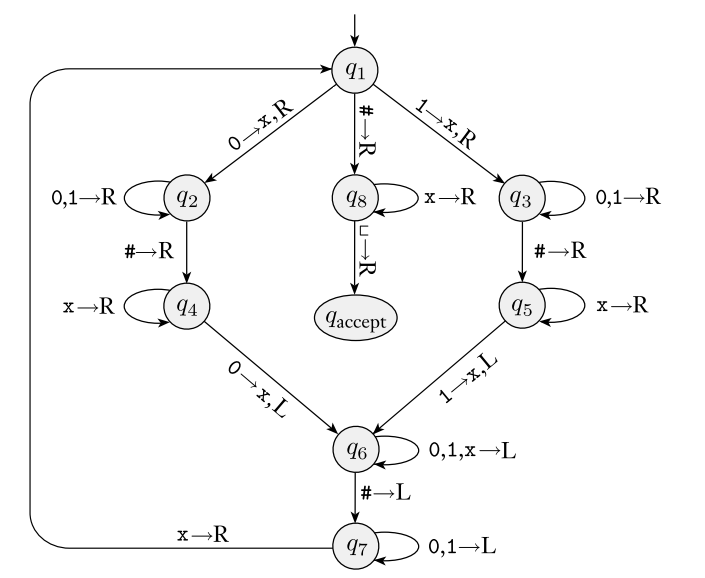
\includegraphics[scale=0.7]{../assets/turing_1.png}
        \end{center}

        To simplify the figure, we don't show the reject state or the transitions going to the reject state. Those transitions occur implicitly whenever a state lacks an outgoing transition for a particular symbol.
    \end{mdframed}

    \item What is $Q$ (the set of states)?
    \begin{mdframed}[]
        \[Q = \{q_1, \dots, q_8, q_{\text{accept}}, q_{\text{reject}}\}\]
    \end{mdframed}

    \item What is $\Sigma$?
    \begin{mdframed}[]
        \[\Sigma = \{\code{0}, \code{1}, \code{\#}\}\]
    \end{mdframed}

    \item What is $\Gamma$?
    \begin{mdframed}[]
        \[\Gamma = \Sigma \cup \{\code{b}, \code{x}\}\]
    \end{mdframed}

    \item Given the string \code{01\#01}, run through the Turing machine. 
    \begin{mdframed}[]
        We begin with the initial configuration. 
        \begin{verbatim}
            State:      q1
            Tape:       0 1 # 0 1
              (Next:)   ^
            Config:     q1 0 1 # 0 1
        \end{verbatim}

        Here, we read in the \code{0} and move to $q_2$, replacing \code{0} with \code{x} and moving the tape to the right. 
        \begin{verbatim}
            State:      q2
            Tape:       x 1 # 0 1
              (Next:)     ^
            Config:     x q2 1 # 0 1
        \end{verbatim}

        At this point, we read in the \code{1} as well (without crossing anything out) and move the tape to the right.  
        \begin{verbatim}
            State:      q2
            Tape:       x 1 # 0 1
              (Next:)       ^
            Config:     x 1 q2 # 0 1
        \end{verbatim}

        For the same reason as above, we read in \code{\#} as well, transitioning to $q_4$ and moving the tape to the right.
        \begin{verbatim}
            State:      q4
            Tape:       x 1 # 0 1
              (Next:)         ^
            Config:     x 1 # q4 0 1
        \end{verbatim}

        Now, we read in the \code{0}, replacing it with a \code{x} and moving the tape left. We also transition to $q_6$. 
        \begin{verbatim}
            State:      q6
            Tape:       x 1 # x 1
              (Next:)       ^
            Config:     x 1 q6 # x 1
        \end{verbatim}

        We read in the \code{\#}, moving the tape to the left and transitioning to $q_7$. 
        \begin{verbatim}
            State:      q7
            Tape:       x 1 # x 1
              (Next:)     ^
            Config:     x q7 1 # x 1
        \end{verbatim}

        We now keep looping at $q_7$ whenever we see a \code{0} or \code{1}. In our case, we only need to read one \code{1}, so we do that, while also moving the tape to the left. 
        \begin{verbatim}
            State:      q7
            Tape:       x 1 # x 1
              (Next:)   ^
            Config:     q7 x 1 # x 1
        \end{verbatim}

        We now read in the \code{x} and transition to $q_1$, moving the tape to the right. 
        \begin{verbatim}
            State:      q1
            Tape:       x 1 # x 1
              (Next:)     ^
            Config:     x q1 1 # x 1
        \end{verbatim}

        Now, we transition to $q_3$, reading in the \code{1} and replacing it with an \code{x} while also moving the tape to the right. 
        \begin{verbatim}
            State:      q3
            Tape:       x x # x 1
              (Next:)       ^
            Config:     x x q3 # x 1
        \end{verbatim}

        We now read in the \code{\#}, moving the tape to the right and transitioning to $q_5$.
        \begin{verbatim}
            State:      q5
            Tape:       x x # x 1
              (Next:)         ^
            Config:     x x # q5 x 1
        \end{verbatim}

        We now read in all of the \code{x}'s, moving the tape to the right. We only do this once as there is only one \code{x} to be read. 
        \begin{verbatim}
            State:      q5
            Tape:       x x # x 1
              (Next:)           ^
            Config:     x x # x q5 1
        \end{verbatim}

        We now read in a \code{1}, replacing it with a \code{x}, transitioning to $q_6$, and moving the tape to the left. 
        \begin{verbatim}
            State:      q6
            Tape:       x x # x x
              (Next:)         ^
            Config:     x x # q6 x x
        \end{verbatim}

        At $q_6$, we keep reading in the \code{x}'s. We only do this once, so we move the tape one to the left. 
        \begin{verbatim}
            State:      q6
            Tape:       x x # x x
              (Next:)       ^
            Config:     x x q6 # x x
        \end{verbatim}

        Now, we transition to $q_7$ since the next symbol is \code{\#}, moving the tape to the left. 
        \begin{verbatim}
            State:      q7
            Tape:       x x # x x
              (Next:)     ^
            Config:     x q7 x # x x
        \end{verbatim}

        We transition to $q_1$, moving the tape to the right. 
        \begin{verbatim}
            State:      q1
            Tape:       x x # x x
              (Next:)       ^
            Config:     x x q1 # x x
        \end{verbatim}

        Since the next symbol to be read is a \code{\#}, we transition to $q_8$, moving the tape to the right. 
        \begin{verbatim}
            State:      q8
            Tape:       x x # x x
              (Next:)         ^
            Config:     x x # q8 x x
        \end{verbatim}

        We now keep reading in any \code{x}'s, moving the tape to the right. This is done twice.
        \begin{verbatim}
            State:      q8
            Tape:       x x # x x
              (Next:)             ^
            Config:     x x # x x q8
        \end{verbatim}

        At this point, we are implicitly at a $\sqcup$. So, we move to $q_{\text{accept}}$. Thus, this string is accepted.
    \end{mdframed}
\end{enumerate}

\end{document}